\section{动态多态性}

因为历史原因,C++一开始只通过结合使用继承和虚函数来支持多态。

\begin{notice}
严格地说,宏也可以认为是静态多态性的早期形式。但这里不对宏进行讨论,因为它们大多与其他语言机制不相关。
\end{notice}

多态设计的艺术包括在相关对象类型中标识一组公共功能,并将它们声明为公共基类中的虚函数接口。

这种设计方法的代表是管理几何图形,并允许以某种方式(例如,在屏幕上)呈现的应用程序。这样的应用程序中,可以识别一个抽象基类(ABC)GeoObj,声明了适用于几何对象的常见操作和属性。然后,特定几何对象的每个具体类都派生自GeoObj(见图18.1):

\begin{center}
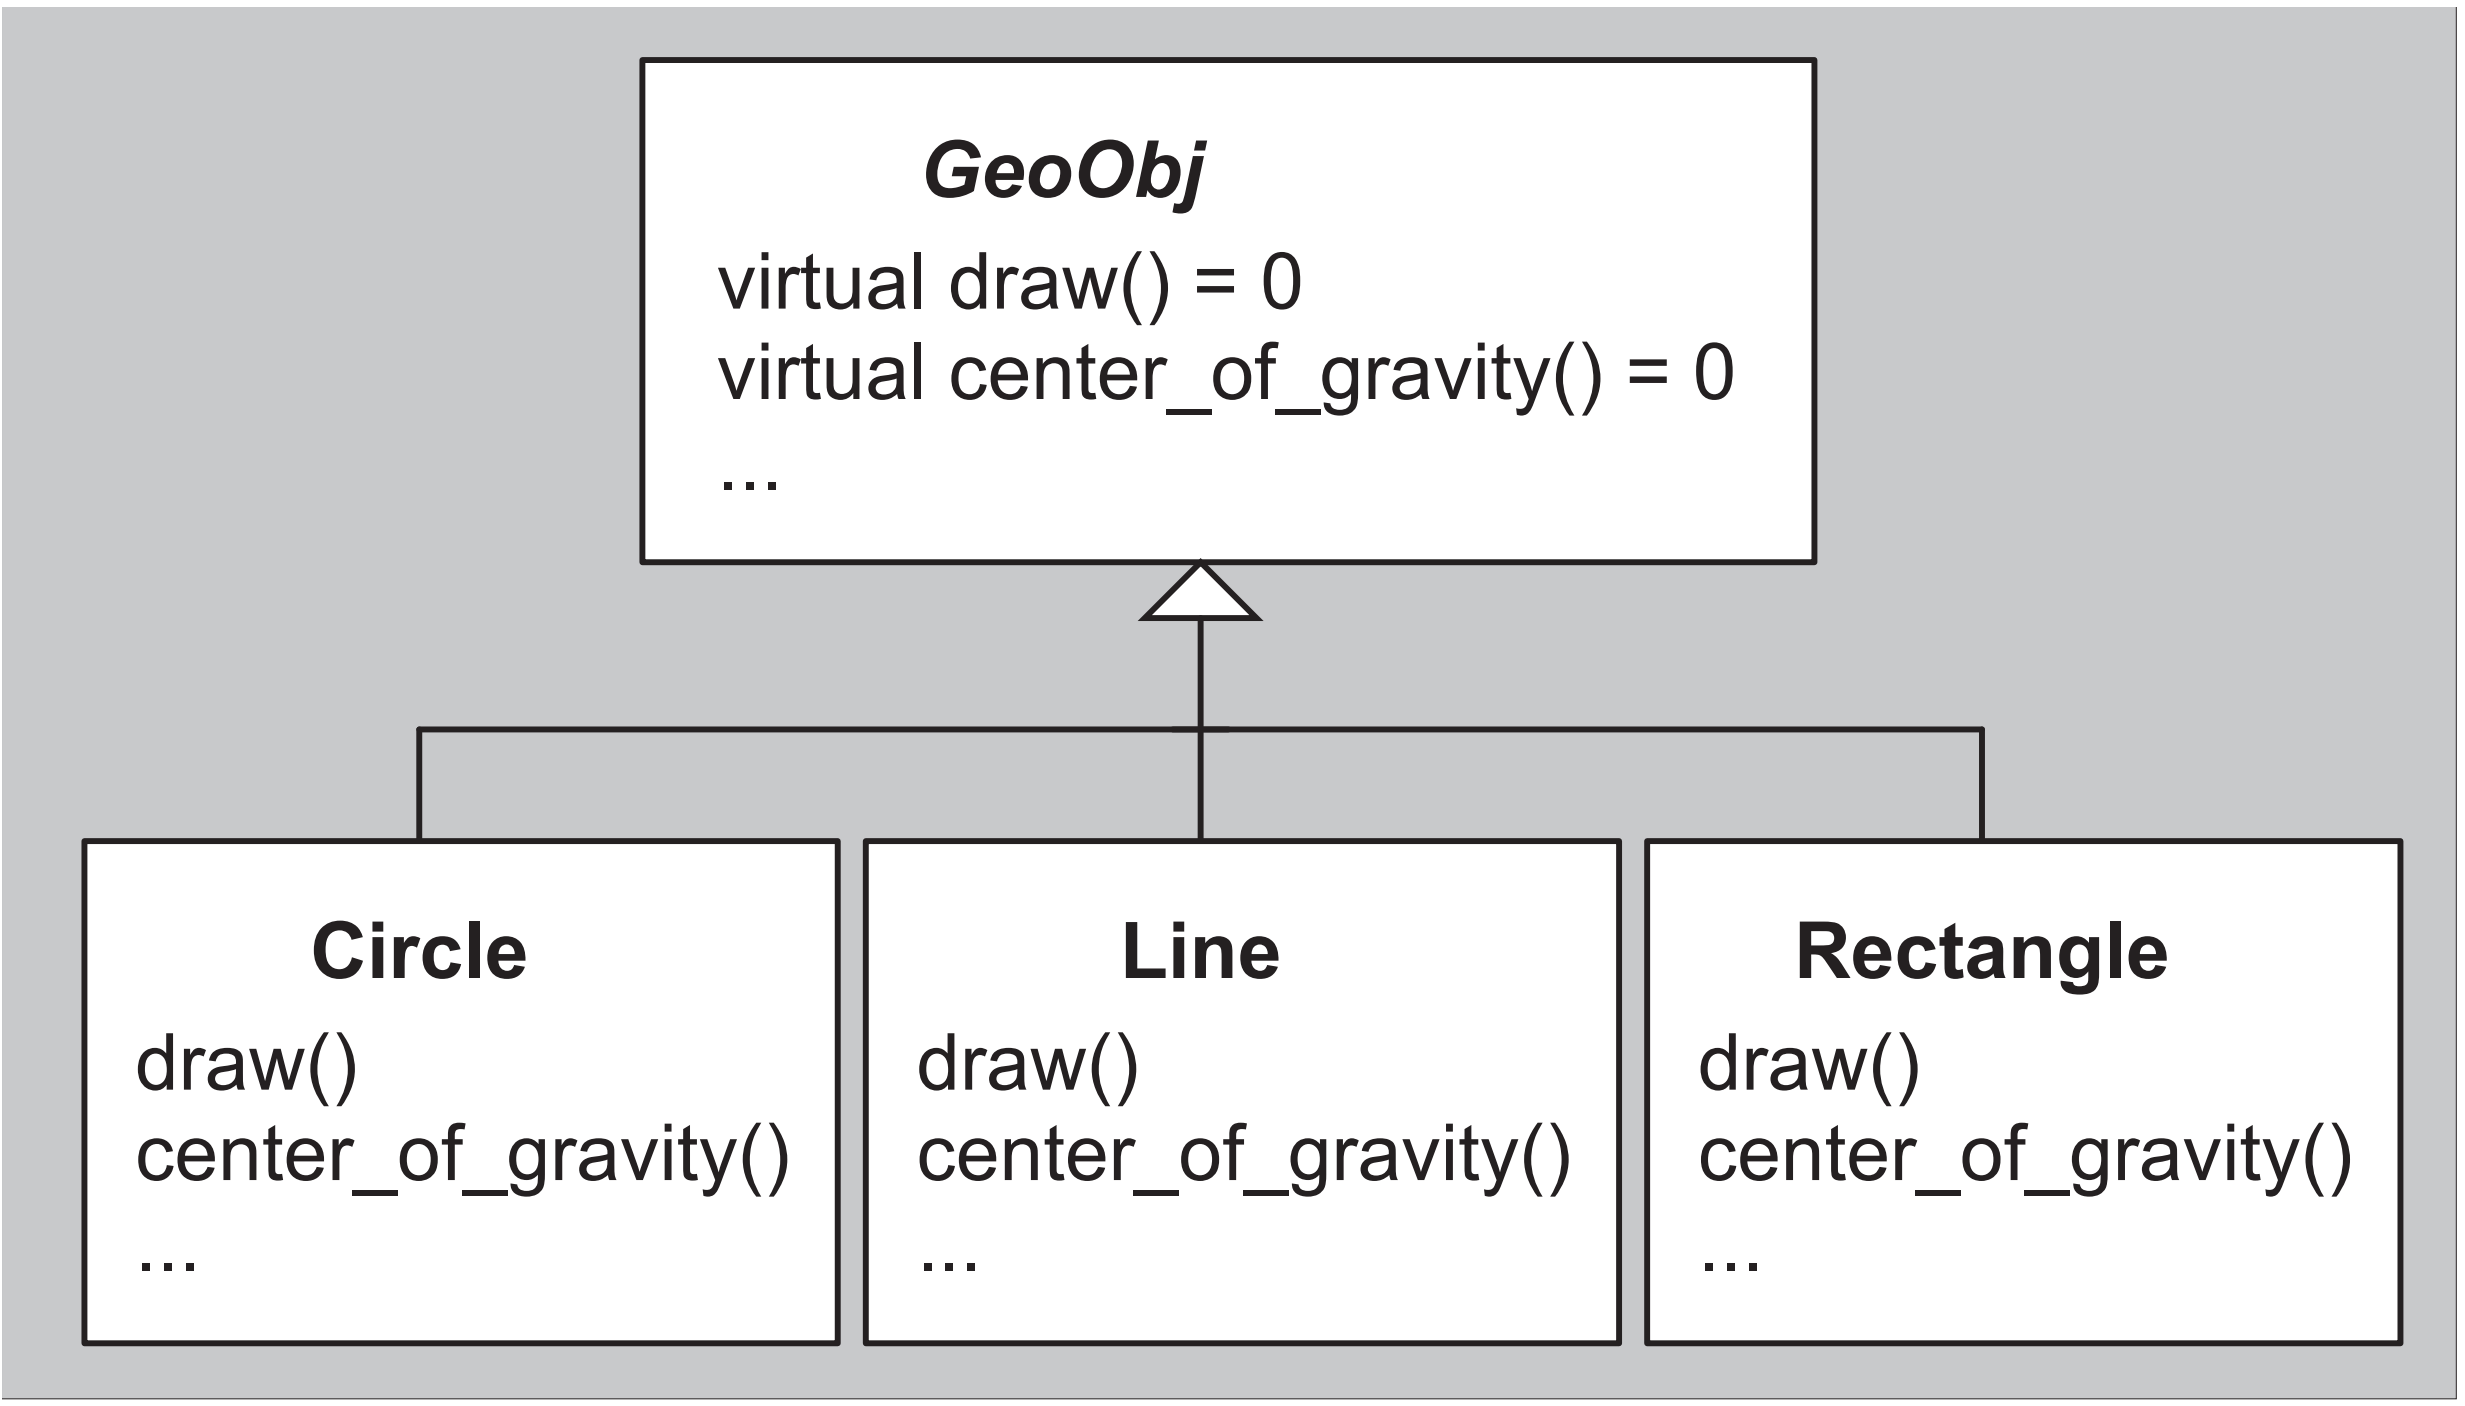
\includegraphics[width=0.8\textwidth]{part3/ch18/images/1.png} \\
图18.1. 通过继承实现的多态性
\end{center}

\filename{poly/dynahier.hpp}
\begin{cpp}
#include "coord.hpp"

// common abstract base class GeoObj for geometric objects
class GeoObj {
	public:
	// draw geometric object:
	virtual void draw() const = 0;
	// return center of gravity of geometric object:
	virtual Coord center_of_gravity() const = 0;
	...
	virtual ~GeoObj() = default;
};

// concrete geometric object class Circle
// - derived from GeoObj
class Circle : public GeoObj {
	public:
	virtual void draw() const override;
	virtual Coord center_of_gravity() const override;
	...
};

// concrete geometric object class Line
// - derived from GeoObj
class Line : public GeoObj {
	public:
	virtual void draw() const override;
	virtual Coord center_of_gravity() const override;
	...
};
...
\end{cpp}

创建具体对象后,外部代码可以使用虚拟函数分派机制,通过引用或指向公共基类的指针来操作这些对象。通过指向基类子对象的指针或引用调用虚成员函数,是实际类型中的相应函数。

具体代码如下:

\filename{poly/dynapoly.hpp}
\begin{cpp}
#include "dynahier.hpp"
#include <vector>

// draw any GeoObj
void myDraw (GeoObj const& obj) {
	obj.draw(); // call draw() according to type of object
}

// compute distance of center of gravity between two GeoObjs
Coord distance (GeoObj const& x1, GeoObj const& x2) {
	Coord c = x1.center_of_gravity() - x2.center_of_gravity();
	return c.abs(); // return coordinates as absolute values
}

// draw heterogeneous collection of GeoObjs
void drawElems (std::vector<GeoObj*> const& elems) {
	for (std::size_type i=0; i<elems.size(); ++i) {
		elems[i]->draw(); // call draw() according to type of element
	}
}

int main() {
	Line l;
	Circle c, c1, c2;
	
	myDraw(l); // myDraw(GeoObj&) => Line::draw()
	myDraw(c); // myDraw(GeoObj&) => Circle::draw()
	
	distance(c1,c2); // distance(GeoObj&,GeoObj&)
	distance(l,c); // distance(GeoObj&,GeoObj&)
	
	std::vector<GeoObj*> coll; // heterogeneous collection
	coll.push_back(&l); // insert line
	coll.push_back(&c); // insert circle
	drawElems(coll); // draw different kinds of GeoObjs
}
\end{cpp}

关键的多态接口是函数draw()和center\_of\_gravity(),二者都是虚成员函数。示例演示了在函数mydraw()、distance()和drawElems()中的用法,后面的函数使用基类型GeoObj中的实现。这种方法的结果是,在编译时通常不知道必须调用哪个版本的draw()或center\_of\_gravity()。但在运行时,将访问虚函数调用的对象的完整动态类型,以调用相应函数。

\begin{notice}
也就是说,多态基类子对象的编码包括一些(大部分是隐藏的)支持运行时分配。
\end{notice}

因此,根据几何对象的实际类型,会执行相应的操作:如果对Line对象调用mydraw(),则表达式obj.draw()会调用Line::draw(),而对Circle对象调用Circle::draw()函数。类似地,使用distance(),调用适合于参数对象的成员函数center\_of\_gravity()。

这种动态多态的特点,可能是处理异构对象集合的能力。drawElems()可以很好的说明:

\begin{cpp}
elems[i]->draw()
\end{cpp}

上述表达式结果调用不同的成员函数,这取决于迭代元素的动态类型。


























